% Dokumentklassen s�ttes til memoir.
% Manual: http://ctan.org/tex-archive/macros/latex/contrib/memoir/memman.pdf
\documentclass[a4paper,oneside,article]{memoir}

\usepackage{pgf}
\usepackage{tikz}
\usepackage{pgfplots}
\usetikzlibrary{arrows,automata}
\usepackage{verbatim}
 
% Danske udtryk (fx figur og tabel) samt dansk orddeling og fonte med
% danske tegn. Hvis LaTeX brokker sig over �, � og � skal du udskifte
% "utf8" med "latin1" eller "applemac". 
\usepackage{inputenc}
\usepackage[danish]{babel}
\usepackage[T1]{fontenc}
 
% Matematisk udtryk, fede symboler, theoremer og fancy ting (fx k�debr�ker)
\usepackage{amsmath,amssymb}
\usepackage{bm}
\usepackage{amsthm}
%\usepackage{mathtools}
 
% Kodelisting. Husk at l�se manualen hvis du vil lave fancy ting.
% Manual: http://mirror.ctan.org/macros/latex/contrib/listings/listings.pdf
\usepackage{listings}
 
% Fancy ting med enheder og datatabeller. L�s manualen til pakken
% Manual: http://www.ctan.org/tex-archive/macros/latex/contrib/siunitx/siunitx.pdf
%\usepackage{siunitx}

% Inds�ttelse af grafik.
\usepackage{graphicx}
\usepackage{float}
\usepackage{caption}
\usepackage{subcaption}
 
% Reaktionsskemaer. L�s manualen for at se eksempler.
% Manual: http://www.ctan.org/tex-archive/macros/latex/contrib/mhchem/mhchem.pdf
%\usepackage[version=3]{mhchem}
%\usepackage[noend]{algpseudocode}
%\usepackage{algorithm}

\usepackage{xcolor,colortbl}

\usepackage{listings}

\definecolor{javared}{rgb}{0.6,0,0} % for strings
\definecolor{javagreen}{rgb}{0.25,0.5,0.35} % comments
\definecolor{javapurple}{rgb}{0.5,0,0.35} % keywords
\definecolor{javadocblue}{rgb}{0.25,0.35,0.75} % javadoc

\lstset{language=Java,
basicstyle=\small, %\ttfamily,
keywordstyle=\color{javapurple}\bfseries,
stringstyle=\color{javared},
commentstyle=\color{javagreen},
morecomment=[s][\color{javadocblue}]{/**}{*/},
numbers=left,
numberstyle=\tiny\color{black},
stepnumber=1,
numbersep=10pt,
tabsize=4,
showspaces=false,
showstringspaces=false}

\newcommand{\notimplies}{%
  \mathrel{{\ooalign{\hidewidth$\not\phantom{=}$\hidewidth\cr$\implies$}}}}

\begin{document}
    \title{Byzantine Agreement - Disposition}
    \author{Lukas Peter J�rgensen, 201206057, DA4
            }
    \maketitle
    
    \chapter{Fault tolerance}
    \section*{Dependability}
    Fault tolerant is strongly related dependable systems.\\
    Dependability is a term that covers a number of useful requirements for distributed systems including:
    \begin{enumerate}
    \item Availability
    \item Reliability
    \item Safety
    \item Maintainability
    \end{enumerate}
    \textbf{Availability} is defined as whether the system is ready to be used immediately.\\
    \textbf{Reliability} is defined as whether a system can run continuously without failure.\\
    \textbf{Safety} is defined as whether something catastrophic happens if the system temporarily fails to operate correctly.\\
    \textbf{Maintainability} is defined as how easy it is to repair a failed system.\\
    The cause of an error is called a fault, a fault might be something simple as overheated-hardware or something more complex as bad weather.\\
    
    \section*{Fault types}
    \begin{itemize}
    \item[Transient] occurs once and then dissappears (e.g. a bird flying through a microwave transmitter)
    \item[Intermittent] occurs, then vanishes for no reason, then reappears etc. Could be a loose contact for example.
    \item[Permanent] occurs and doesn't go away, could be software bug, overloaded hardware etc.
    \end{itemize}
    \begin{figure}[H]
    \centering
    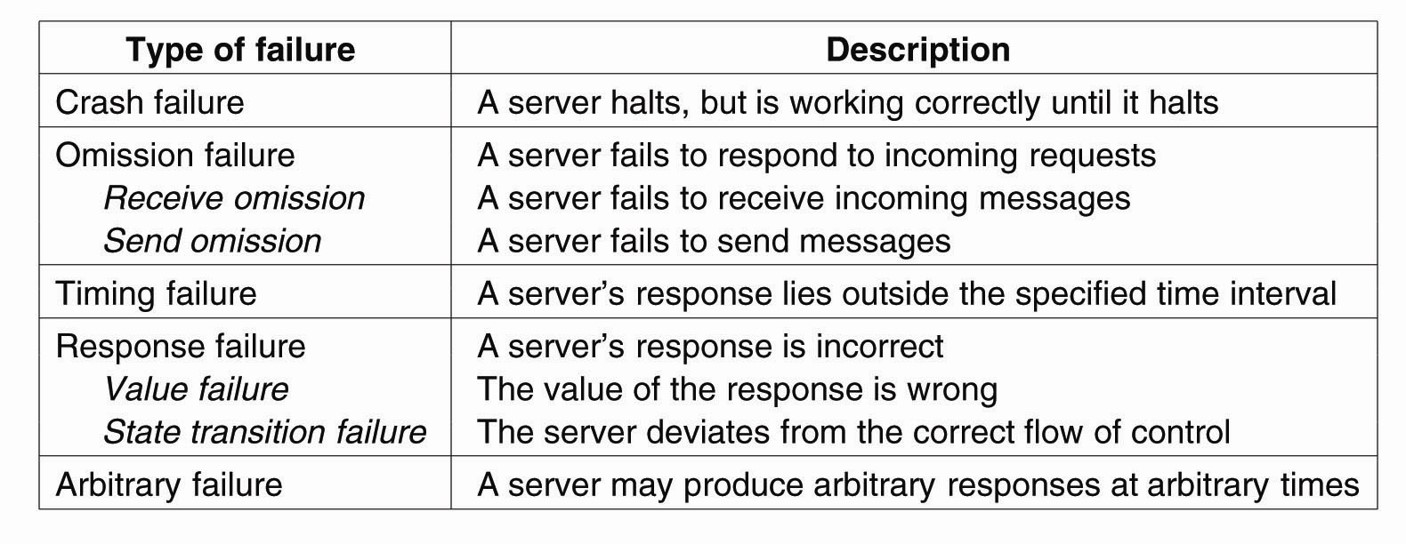
\includegraphics[width=\textwidth]{Media/FailTypes.jpg}
    \end{figure}
    
    \section*{Byzantine failures}
    Also known as arbitary failures, the server might be spitting out arbitrary output, or worse yet it might do it intentionally.
    
    \chapter{Redundancy masking}
    If a system is to be fault tolerant, the best way is to try to hide the occurrence of failures from other processes.\\
    Redundancy is the key technique to achieve this, there are 3 kinds of redundancies:
    \begin{itemize}
    \item Information redundancy
    \item Time redundancy
    \item Physical redundancy
    \end{itemize}
    
    \section*{Information redundancy}
    With information redundancy, you can avoid some issues by providing extra information, e.g. by sending some extra bits to allow recovery from garbled bits.
    
    \section*{Time redundancy}
    With time redundancy, an action is performed and then if need be it is performed again.
    
    \section*{Physical redundancy}
    Add more machines, so you can allow more of them to crash without comprimising the system.
    
    \chapter{Two-army problem}
    \textbf{Agreement not possible.}
    
    \chapter{Byzantine generals problem}
    $2k+1$ correctly functioning processes must be present.\\
    They only have to reach consensus on the nonfaulty values.
\end{document}